\documentclass[12pt,letterpaper]{article}
\usepackage{graphicx,textcomp}
\usepackage{natbib}
\usepackage{setspace}
\usepackage{fullpage}
\usepackage{color}
\usepackage[reqno]{amsmath}
\usepackage{amsthm}
\usepackage{fancyvrb}
\usepackage{amssymb,enumerate}
\usepackage[all]{xy}
\usepackage{endnotes}
\usepackage{lscape}
\newtheorem{com}{Comment}
\usepackage{float}
\usepackage{hyperref}
\newtheorem{lem} {Lemma}
\newtheorem{prop}{Proposition}
\newtheorem{thm}{Theorem}
\newtheorem{defn}{Definition}
\newtheorem{cor}{Corollary}
\newtheorem{obs}{Observation}
\usepackage[compact]{titlesec}
\usepackage{dcolumn}
\usepackage{tikz}
\usetikzlibrary{arrows}
\usepackage{multirow}
\usepackage{xcolor}
\newcolumntype{.}{D{.}{.}{-1}}
\newcolumntype{d}[1]{D{.}{.}{#1}}
\definecolor{light-gray}{gray}{0.65}
\usepackage{url}
\usepackage{listings}
\usepackage{color}

\definecolor{codegreen}{rgb}{0,0.6,0}
\definecolor{codegray}{rgb}{0.5,0.5,0.5}
\definecolor{codepurple}{rgb}{0.58,0,0.82}
\definecolor{backcolour}{rgb}{0.95,0.95,0.92}

\lstdefinestyle{mystyle}{
	backgroundcolor=\color{backcolour},   
	commentstyle=\color{codegreen},
	keywordstyle=\color{magenta},
	numberstyle=\tiny\color{codegray},
	stringstyle=\color{codepurple},
	basicstyle=\footnotesize,
	breakatwhitespace=false,         
	breaklines=true,                 
	captionpos=b,                    
	keepspaces=true,                 
	numbers=left,                    
	numbersep=5pt,                  
	showspaces=false,                
	showstringspaces=false,
	showtabs=false,                  
	tabsize=2
}
\lstset{style=mystyle}
\newcommand{\Sref}[1]{Section~\ref{#1}}
\newtheorem{hyp}{Hypothesis}


\title{Problem Set 4/}
\date{Zengyuan Zhao / zhaoze@tcd.ie}
\author{Quant Methods 1/Due: November 18, 2024}


\begin{document}
	\maketitle
	\section*{Instructions}
	\begin{itemize}
		\item Please show your work! You may lose points by simply writing in the answer. If the problem requires you to execute commands in \texttt{R}, please include the code you used to get your answers. Please also include the \texttt{.R} file that contains your code. If you are not sure if work needs to be shown for a particular problem, please ask.
		\item Your homework should be submitted electronically on GitHub.
		\item This problem set is due before 23:59 on Monday November 18, 2024. No late assignments will be accepted.
	\end{itemize}



	\vspace{.5cm}
\section*{Question 1: Economics}
\vspace{.25cm}
\noindent 	
In this question, use the \texttt{prestige} dataset in the \texttt{car} library. First, run the following commands:

\begin{verbatim}
install.packages(car)
library(car)
data(Prestige)
help(Prestige)
\end{verbatim} 


\noindent We would like to study whether individuals with higher levels of income have more prestigious jobs. Moreover, we would like to study whether professionals have more prestigious jobs than blue and white collar workers.

\newpage
\begin{enumerate}
	
	\item [(a)]
	Create a new variable \texttt{professional} by recoding the variable \texttt{type} so that professionals are coded as $1$, and blue and white collar workers are coded as $0$ (Hint: \texttt{ifelse}).
		\lstinputlisting[language=R, firstline=1, lastline=10]{PS04_answersZYZ.R}
		To better inspect the changed dataframe, I set the number of rows to 30.\\
		\begin{figure}[h!]
			\caption{\footnotesize{The first 30 rows of the data frame}}
			\vspace{.2cm}
			\centering
			\label{fig:1.1}
			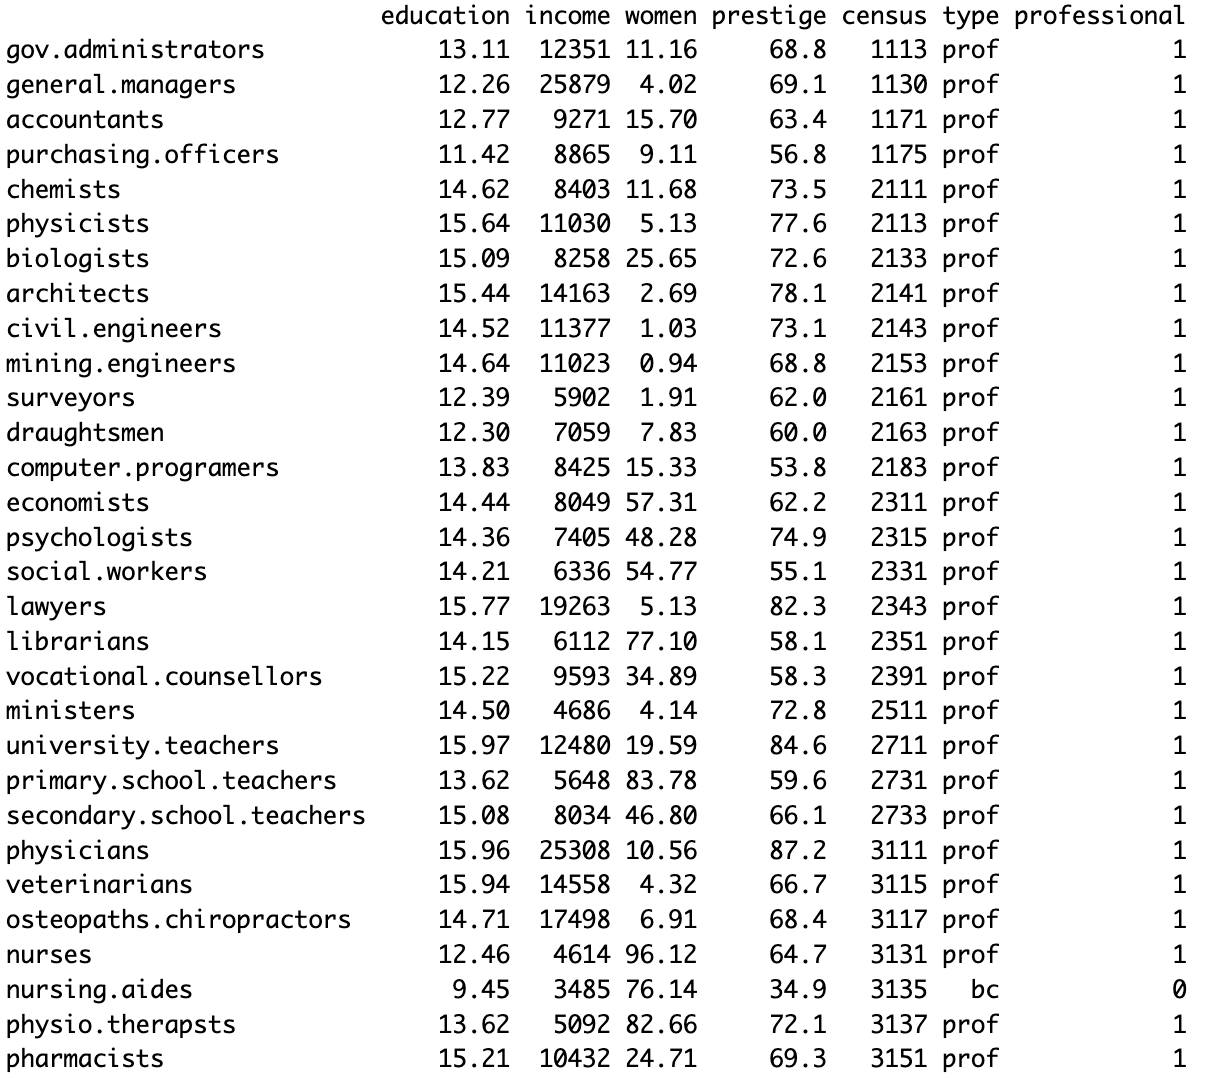
\includegraphics[width=0.9\textwidth]{Prestige.png}
		\end{figure}
	\vspace{15cm}
	\item [(b)]
	Run a linear model with \texttt{prestige} as an outcome and \texttt{income}, \texttt{professional}, and the interaction of the two as predictors (Note: this is a continuous $\times$ dummy interaction.)
	\lstinputlisting[language=R, firstline=11, lastline=15]{PS04_answersZYZ.R}
	\begin{figure}[h!]
		\caption{\footnotesize{The linear model between prestige,income, professional, and the interaction}}
		\vspace{.2cm}
		\centering
		\label{fig:1.2}
		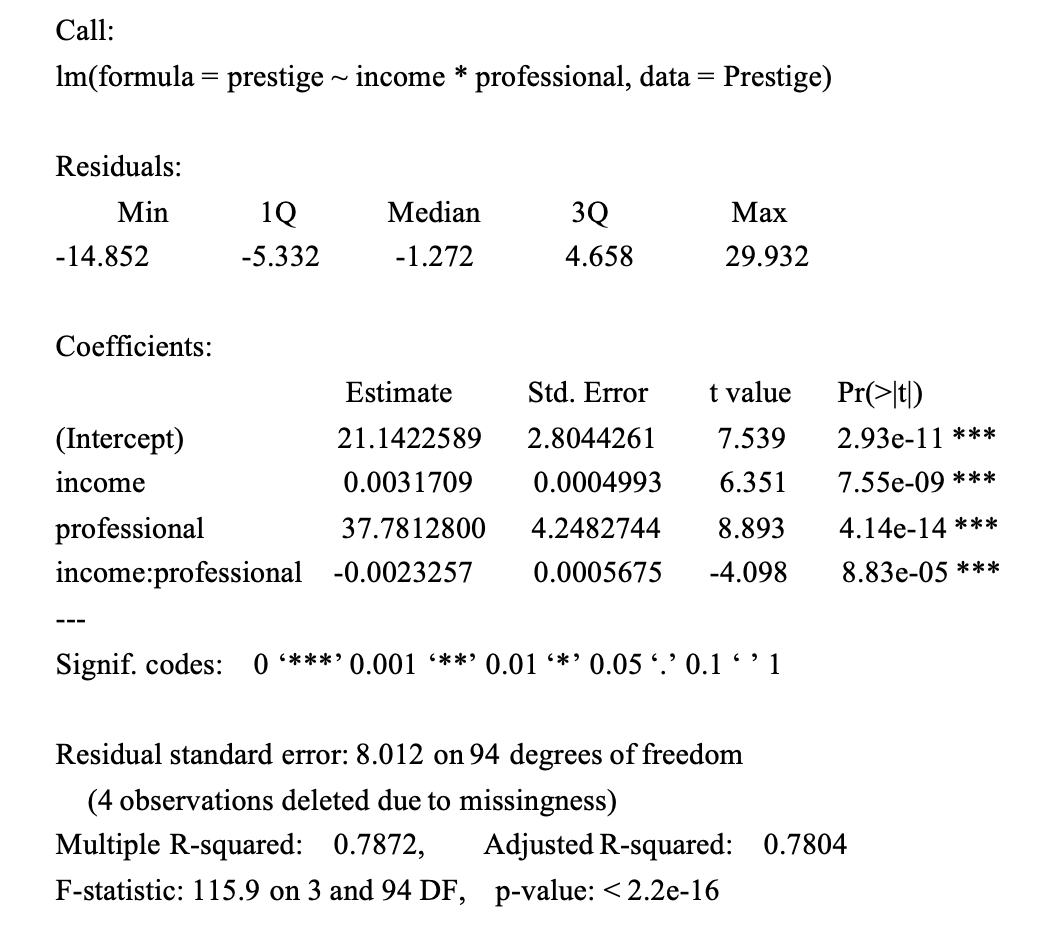
\includegraphics[width=0.7\textwidth]{summary.png}
	\end{figure}
	\item [(c)]
	Write the prediction equation based on the result.
	\lstinputlisting[language=R, firstline=16, lastline=25]{PS04_answersZYZ.R}
	The code output is:\\
	
	"prestige =  21.1422588538203 + 0.00317090909728508 * income + 37.7812799549884 * professional -0.00232570911767063 * income * professional"\\

	Keep the equation to 5 decimal places:\\

	prestige =  21.14226 + 0.00317 * income + 37.78128 * professional -0.00233 * income * professional\\

	\item [(d)]
	Interpret the coefficient for \texttt{income}.	\vspace{1cm}
	
	Ignoring the interaction effect and the coefficient of professional(coefficient=0), the coefficient of income reflects the direct impact of income on prestige. Specifically, when income increases by one unit, prestige is expected to increase by 0.0031709 units, which is the marginal effect under the premise that the level of professional remains unchanged.\\
	
	However, the interaction between income and professional cannot be ignored. The coefficient of the interaction term -0.0023257 reveals how the impact of income on prestige changes with changes in the level of professional. Specifically, every time professional increases by one unit, the marginal effect of income on prestige will decrease by 0.0023257 units. This shows that as professional increases, the reinforcing effect of income on prestige gradually weakens.\\
	\vspace{1cm}	
	\item [(e)]
	Interpret the coefficient for \texttt{professional}.	\vspace{1cm}
	
	When the interaction between income and professional is ignored(coefficient=0), the coefficient of professional will directly reflect its marginal impact on prestige. Specifically, the coefficient of professional is 37.7812800, which means that when income remains unchanged, for every unit increase in professional, prestige will increase by an average of 37.7812800 units. This is a significant positive effect.\\
	
	The interaction between income and professionalism is inevitable. The existence of the interaction term means that the impact of professional on prestige does not exist in isolation, but will be moderated by income level. Specifically, the interaction term coefficient -0.0023257 reveals that as professionalism increases, the marginal effect of income on prestige will weaken.\\

	\item [(f)]
	What is the effect of a \$1,000 increase in income on prestige score for professional occupations? In other words, we are interested in the marginal effect of income when the variable \texttt{professional} takes the value of $1$. Calculate the change in $\hat{y}$ associated with a \$1,000 increase in income based on your answer for (c).
	
	The equation of question C is known to be:\\
	prestige = 21.1423 + 0.00317 * income + 37.7812 * professional -0.00233 * income * professional\\
	According to the question requirements, professional is 1, and the simplified equation is:\\
	prestige=58.9235+0.000845 * income\\
	Since the change value of income = 1000,\\
	therefore the margin effect of prestige = (0.003171 - 0.002326) * 1000 = 0.845\\
	According to the calculation process, we can conclude that when the professional variable value is 1:\\
	Income marginal value = (income coefficient + interaction coefficient) * income change value\\
	Run this formula in R:\\
	\lstinputlisting[language=R, firstline=26, lastline=30]{PS04_answersZYZ.R}

	The code output is:\\
	
	"When professional is 1 and income increases 1000 , the marginal effect of income is 0.845199979614447"
	
	\item [(g)]
	What is the effect of changing one's occupations from non-professional to professional when her income is \$6,000? We are interested in the marginal effect of professional jobs when the variable \texttt{income} takes the value of $6,000$. Calculate the change in $\hat{y}$ based on your answer for (c).
	
	I need to calculate the prestige of professionals and non-professionals respectively, and calculate the marginal difference between them. That is, substitute income=6000, professional=1 and income=6000, professional=0 into the formula respectively, and finally calculate the difference between the prestige of professionals and non-professionals. The calculation of this question will be completed in R.\\
	
	\lstinputlisting[language=R, firstline=31, lastline=41]{PS04_answersZYZ.R}
	
	The code output is:\\
	
	"When a person's income is 6000 switching from a nonprofessional to a professional occupation will result in an increase in her prestige of approximately 23.8270252489646 units."
\end{enumerate}

\newpage

\section*{Question 2: Political Science}
\vspace{.25cm}
\noindent 	Researchers are interested in learning the effect of all of those yard signs on voting preferences.\footnote{Donald P. Green, Jonathan	S. Krasno, Alexander Coppock, Benjamin D. Farrer,	Brandon Lenoir, Joshua N. Zingher. 2016. ``The effects of lawn signs on vote outcomes: Results from four randomized field experiments.'' Electoral Studies 41: 143-150. } Working with a campaign in Fairfax County, Virginia, 131 precincts were randomly divided into a treatment and control group. In 30 precincts, signs were posted around the precinct that read, ``For Sale: Terry McAuliffe. Don't Sellout Virgina on November 5.'' \\

Below is the result of a regression with two variables and a constant.  The dependent variable is the proportion of the vote that went to McAuliff's opponent Ken Cuccinelli. The first variable indicates whether a precinct was randomly assigned to have the sign against McAuliffe posted. The second variable indicates
a precinct that was adjacent to a precinct in the treatment group (since people in those precincts might be exposed to the signs).  \\

\vspace{.5cm}
\begin{table}[!htbp]
	\centering 
	\textbf{Impact of lawn signs on vote share}\\
	\begin{tabular}{@{\extracolsep{5pt}}lccc} 
		\\[-1.8ex] 
		\hline \\[-1.8ex]
		Precinct assigned lawn signs  (n=30)  & 0.042\\
		& (0.016) \\
		Precinct adjacent to lawn signs (n=76) & 0.042 \\
		&  (0.013) \\
		Constant  & 0.302\\
		& (0.011)
		\\
		\hline \\
	\end{tabular}\\
	\footnotesize{\textit{Notes:} $R^2$=0.094, N=131}
\end{table}

\vspace{.5cm}
\begin{enumerate}
	\item [(a)] Use the results from a linear regression to determine whether having these yard signs in a precinct affects vote share (e.g., conduct a hypothesis test with $\alpha = .05$).
	
	According to the linear regression results, the coefficient of "Precinct assigned lawn signs (n=30)" is 0.042, and the standard error is 0.016. The coefficient of "Precinct adjacent to lawn signs (n=76)" is also 0.042, and the standard error is 0.013. The constant term (intercept) is 0.302, and its standard error is 0.011.\\
	
	{\large Setting hypothesis\\}
	Null hypothesis (H0): Placing campaign placards has no effect on voting proportion, that is, the coefficient of the Precinct assigned lawn signs variable is equal to 0.\\
	Alternative hypothesis (H1): Placing campaign placards has an effect on voting proportion, that is, the coefficient of the Precinct assigned lawn signs variable is not equal to 0.\\
	
	Next, I will use the t-test method in R to judge whether to accept the null hypothesis.\\
	
	\lstinputlisting[language=R, firstline=42, lastline=56]{PS04_answersZYZ.R}
	The code output is:\\
	
	"At a significance level of  0.05 , the null hypothesis is rejected. So, there is sufficient evidence that put these yard signs in a precinct has an effect on the vote share."\\
	
	The t-test showed that the t-value(2.625) was greater than the critical value(1.978671), so the null hypothesis was rejected, indicating that there was sufficient evidence to show that placing signs in the  precinct had an impact on the voting share.\\
	\newpage		
	\item [(b)]  Use the results to determine whether being
	next to precincts with these yard signs affects vote
	share (e.g., conduct a hypothesis test with $\alpha = .05$).
	
	{\large Setting hypothesis\\}
	Null Hypothesis (H{\small a}): Being next to precincts with yard signs does not affect vote share.\\
	Alternative Hypothesis(H{\small b}): Being next to precincts with yard signs does affect vote share.\\
	
	Next, I will use the t-test method in R to judge whether to accept the null hypothesis.\\
	
	\lstinputlisting[language=R, firstline=57, lastline=69]{PS04_answersZYZ.R}
	The code output is:\\
	
	"At a significance level of  0.05 , the null hypothesis is rejected. So, there is sufficient evidence that being next to precincts with these yard signs has an effect on the vote share."\\
	
	The t-test showed that the t-value (3.230769) was greater than the critical value (1.978671), so the null hypothesis was rejected, indicating that there was sufficient evidence to show that being near the precinct with signs had an impact on the voting share.\\

	\item [(c)] Interpret the coefficient for the constant term substantively.

In the framework of linear regression analysis, the coefficient of the constant term (or intercept term) represents the conditional expected value of the dependent variable "vote share" when all independent variables take their baseline values ( usually 0, which is the case when the binary variables are not activated or do not exist). In this particular problem, the constant term coefficient (0.302) represents the expected level of vote share in the corresponding constituency when the two binary independent variables "constituency assigned with propaganda signs" and "constituency adjacent to propaganda signs" are both set to 0 (that is, when neither of these two conditions is met).

At the same time, the standard error of the constant term coefficient is 0.011, which is relatively small, indicating that the estimate of the constant term coefficient is relatively stable and reliable. The closer the standard error is to 0, it usually means that the estimation is more precise and the confidence interval is narrower, so we can be more confident in the estimate of the constant term coefficient.\\

	\item [(d)] Evaluate the model fit for this regression.  What does this	tell us about the importance of yard signs versus other factors that are not modeled?
	
R², the coefficient of determination, is the core indicator for measuring the fitting effect of the regression model. It represents the proportion of variability in the dependent variable explained by the independent variables in the model. R² = 0.094: This shows that the independent variable in the model (i.e., constituencies assigned propaganda signs versus constituencies adjacent to propaganda signs) can only explain a small 9.4 of the total variation in vote share. Therefore, the model's ability to explain the data is weak.\\

The remaining 90.6 of the variability is attributed to various other factors not included in the model. Although the two variables of precinct assigned signs and precinct adjacent to signs have a statistically significant relationship with the opponent's vote share, they account for a relatively small proportion of the total variation in vote share explained, only 9.4. This suggests that in addition to these two variables, there are other more important factors affecting vote share.\\

Other factors may include the candidate's financial investment, the candidate's policy advocacy, the voter's age, education level, etc.
\end{enumerate}  


\end{document}
